\documentclass{article}
\usepackage[utf8]{inputenc}
\usepackage{graphicx}
\usepackage{geometry}
\usepackage{amsmath}
\usepackage{amsfonts}
\usepackage{float}
\usepackage{caption}
\usepackage{subcaption}
\usepackage{enumitem}

\geometry{left=25mm, top=25mm, right=25mm, bottom=25mm}

\title{PHY407 Lab 8}
\author{Pierino Zindel (1002429703) and Hayden Johnson (1002103537)}
\date{November 2, 2018}

\begin{document}

\maketitle

\noindent \textbf{Distribution of work:} Question 1 was completed by Hayden. Question 2 and 3 were completed by Pierino.

\section{Temperature Distribution in a Heat Conductor}

\subsection{Part b)}

We seek to evaluate the impact of overrelaxation by examining the solution to the heat equation with the given boundary conditions after 100 iterations using the Gauss-Seidel method with both regular relaxation ($w=0$) and overrelaxation with $w=0.9$. 

We did this by making the simple modification to our code from part a) to run the loop which computes new values of the temperature iteratively only 100 times, instead of until a target precision was reached. A plot of the temperature after 100 iterations with $w=0.0$, which corresponds to regular relaxation, is shown in figure \ref{fig:1b_w=0.0}, while a plot of the temperature of 100 iterations with $w=0.9$, which is an example of overrelaxation, is shown in figure \ref{fig:1b_w=0.9}. 

\begin{figure}[H]
	\centering
	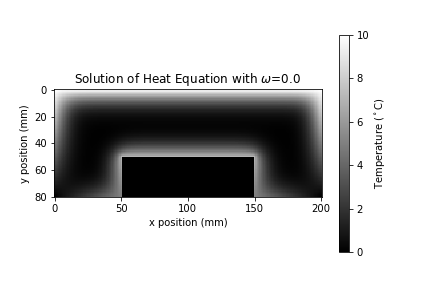
\includegraphics[width=0.8\textwidth]{../images/q1_b_0p0.png}
	\caption{Plot of temperature distribution after 100 iterations using Gauss-Seidel method, with regular relaxation ($w=0.0$).}
	\label{fig:1b_w=0.0}
\end{figure}

The two solutions are qualitatively quite different; in the case of regular relaxation (figure \ref{fig:1b_w=0.0}), the initial value of $T\approx 0$ still persists throughout much of the interior of the domain after 100 iterations, and we can see that the heat from the non-zero boundaries is beginning to permeate gradually through towards the interior of the domain, but it has not gotten very far. The drop off from the non-zero boundaries moving in towards the interior is thus quite steep.

Contrast this with the case of overrelaxation (figure \ref{fig:1b_w=0.9}), where the solution after the same number of iterations (100) looks quite smooth throughout the whole of the domain, and we can see that the heat from the boundaries has penetrated all the way through to the center of the domain. Thus, we can conclude that the overrelaxation Gauss-Seidel method has gotten far closer to the steady-state solution than regular relaxation Gauss-Seidel method has in the same number of iterations, and thus that the overrelaxation method should also converge to the steady-state solution more quickly than the regular relaxation method. Given what we know about how overrelaxation tries to accelerate the convergence by ``overestimating" the correction at each iteration, this makes perfect sense.


\begin{figure}[H]
	\centering
	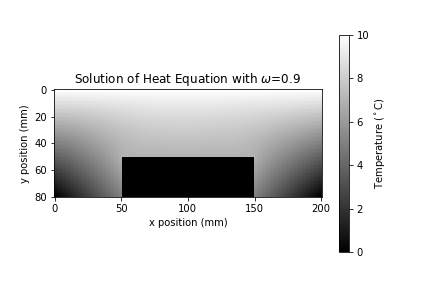
\includegraphics[width=0.8\textwidth]{../images/q1_b_0p9.png}
	\caption{Plot of temperature distribution after 100 iterations using Gauss-Seidel method, with overrelaxation ($w=0.9$).}
	\label{fig:1b_w=0.9}
\end{figure}

\subsection{Part c)}

We seek to calculate the steady-state temperature at each grid point to a precision of $10^{-6}$ $^\circ C$, using overrelaxation Gauss-Seidel with $w=0.9$, and also animate the process of iteratively solving the equation.

We adapted our program from part a) to use the Gauss-Seidel overrelaxation method with $w=0.9$ to iteratively solve the heat equation on the specified domain with the given boundary conditions, and to proceed until the maximum change in value between one iteration and the next at any single point in the domain was less than the specified target precision of $10^{-6}$ $^\circ C$. Doing this, we found the converged solution plotted in figure \ref{fig:1c}. Notice that this looks quite similar to the solution found after 100 iterations using the overrelaxation method in part b) (figure \ref{fig:1b_w=0.9}), indicating that the answer was already quite close after only that many iterations.

From the animation, it was clear that, before the solution got close to converging, the values of the temperature in the array were not symmetric about the line $x=10$, even though the domain and boundary conditions being symmetric about this line imply that the final solution should be too (as indeed it is). This temporary asymmetry is consequence of the way in which the Gauss-Seidel method updates the temperature values, moving in this case from left to right and top to bottom, and at each step using the most recent value available. This means that when the new value at each point is computed, it uses values from the current iteration from its neighbours above and to the left of it, while it uses values from the old iteration from its neighbours below and to the right of it. Hence, information initially can propagate much more quickly downwards and to the right than it does in the opposite directions - in theory, a large value at the top left of the grid could see its influence spread all the way to the bottom right in the course of a single iteration, whereas information can propagate from right to left and from bottom to top at a maximum speed of a single grid square per iteration. Eventually, as we get nearer and nearer to the converged solution, the small differences between the current values and the equilibrium values mean that there are no longer any large discrepancies to be propagated, and this asymmetry ceases to matter, yielding our (approximately) correct converged solution.

Using the coordinate system as it is defined by the axes in figure \ref{fig:1c}, the value of the converged solution at $x=2.5$cm, $y=1.0$cm is $T = 9.030218 ^\circ$C. Note that, if we instead define the y axis to be increasing upwards starting from the bottom left corner (i.e. like a regular Cartesian coordinate system), $y=1.0$cm corresponds to $y=7.0$cm on the figure axis, which gives a value of $T = 3.435926 ^\circ$C.

\begin{figure}[H]
	\centering
	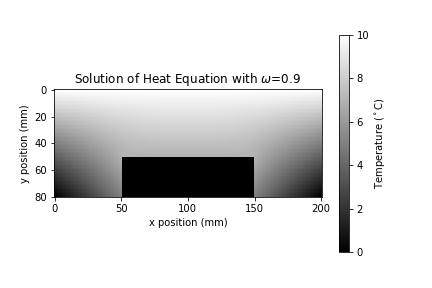
\includegraphics[width=0.8\textwidth]{../images/q1_c.png}
	\caption{Plot of temperature distribution created using Gauss-Seidel method, with overrelaxation ($w=0.9$), with a target precision of $1.0\times 10^{-6}$.}
	\label{fig:1c}
\end{figure}


\section{FTCS solution of the wave equation}
For this question we desire to solve the wave equation using the FTCS method. The FTCS equations used for the solution were

\begin{equation}
	\phi(x, t+h) = \phi(x,t)+h\psi(x,t)
\end{equation}

\begin{equation}
	\psi(x, t+h) = \psi(x,t)+h\frac{v^2}{a^2}(\phi(x+a,t)+\phi(x-a,t)-2\phi(x,t))
\end{equation}

with the initial conditions that $\phi(x)=0$ and 

\begin{equation}
	\psi(x) = C\frac{x(L-x)}{L^2}exp(-\frac{(x-d)^2}{2\sigma^2})
\end{equation}

where $L=1.0m$, $d=0.1m$, $C=1.0m/s$, $\sigma=0.3m$. 

The conditions used to get our solution were a step of $h=10^{-6}s$, number of points $N=100$, and spacing $a=L/N$. The solution was plotted from $t=0.0s$ to $t=0.101s$ to observe how the solution using FTCS becomes unstable. The initial solution at a time of $t=2ms$ is shown is figure \ref{fig:q2_2}. From here the FTCS method seems to give us a good stable solution until roughly $t=71ms$ when we can clearly see the instability of the method begin (see figure \ref{fig:q2_71}). Then after another $24ms$ the solution instability grows considerably to significant value where the actual solution becomes distorted, as can be see in figure \ref{fig:q2_95}. And at the end of our running time of $t=101ms$ we can see in figure \ref{fig:q2_101} that the instability of the FTCS method has out grown our initial solution and thus the result that the FTCS method gives us for the wave equation for long enough running time is incomprehensible in terms of the actual solution. 

\begin{figure}[H]
	\centering
	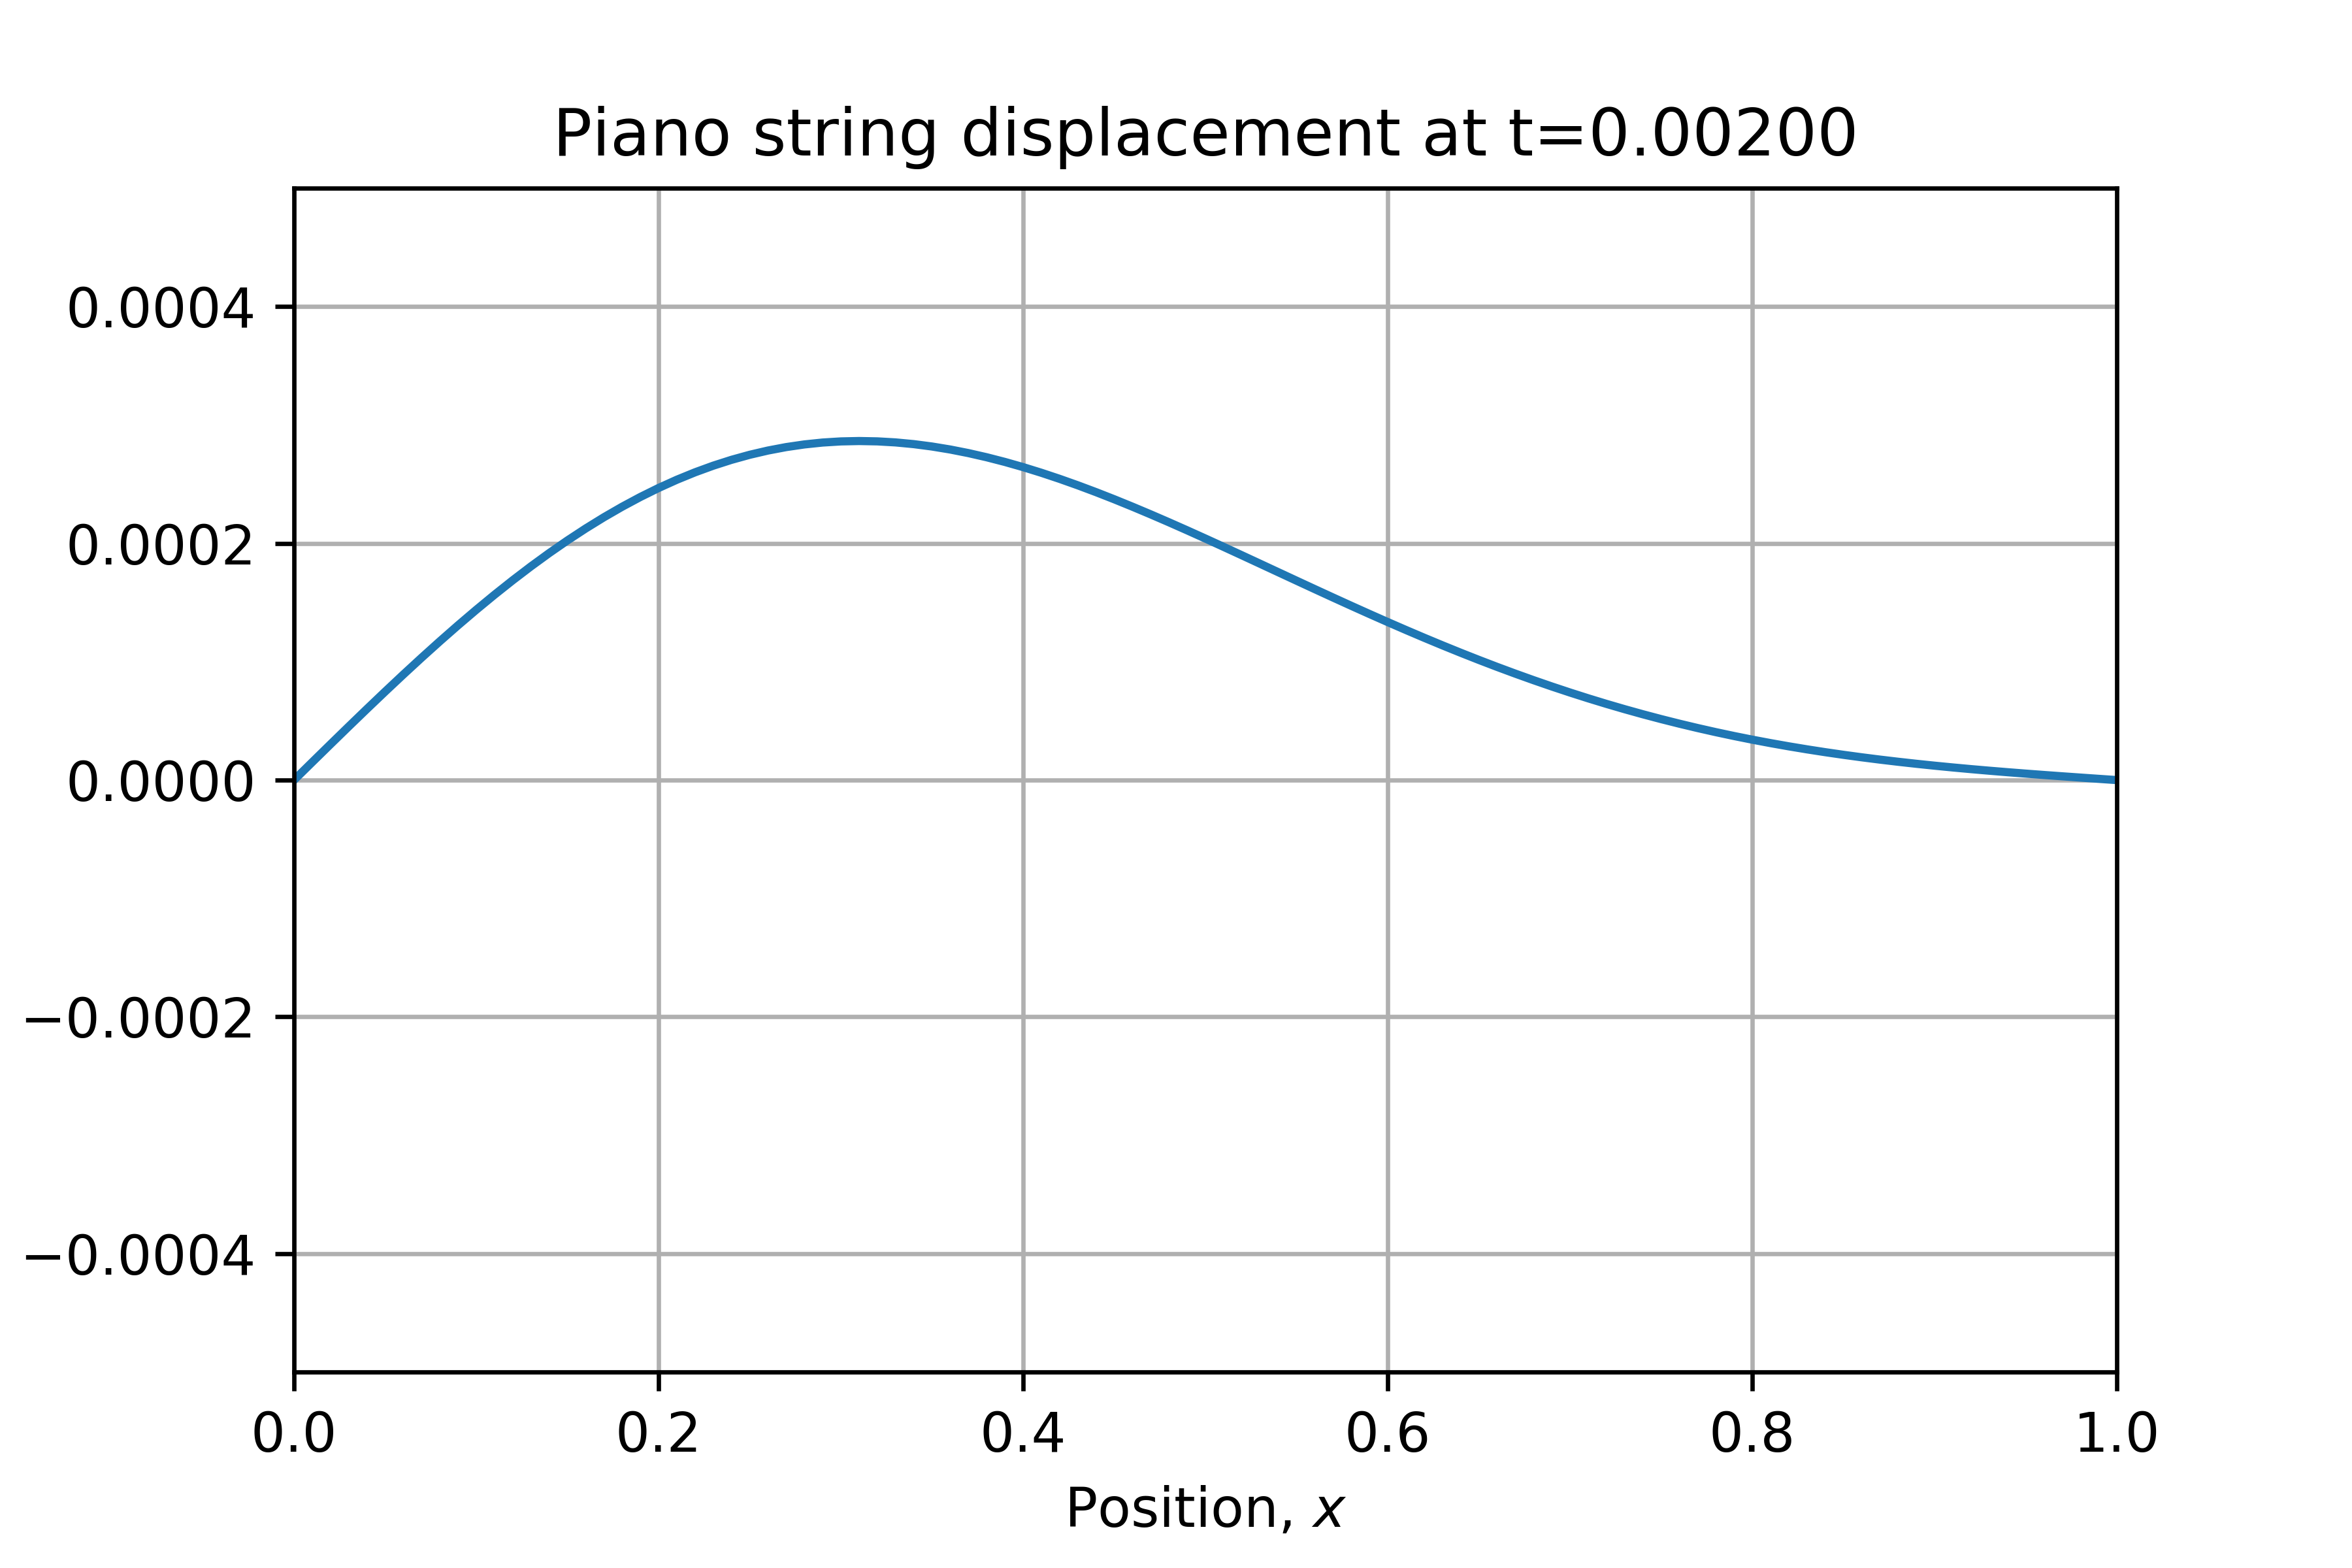
\includegraphics[width=0.8\textwidth]{../images/q2_plot_2.png}
	\caption{Plot of the piano string displacement at a time of 2ms.}
	\label{fig:q2_2}
\end{figure}

\begin{figure}[H]
	\centering
	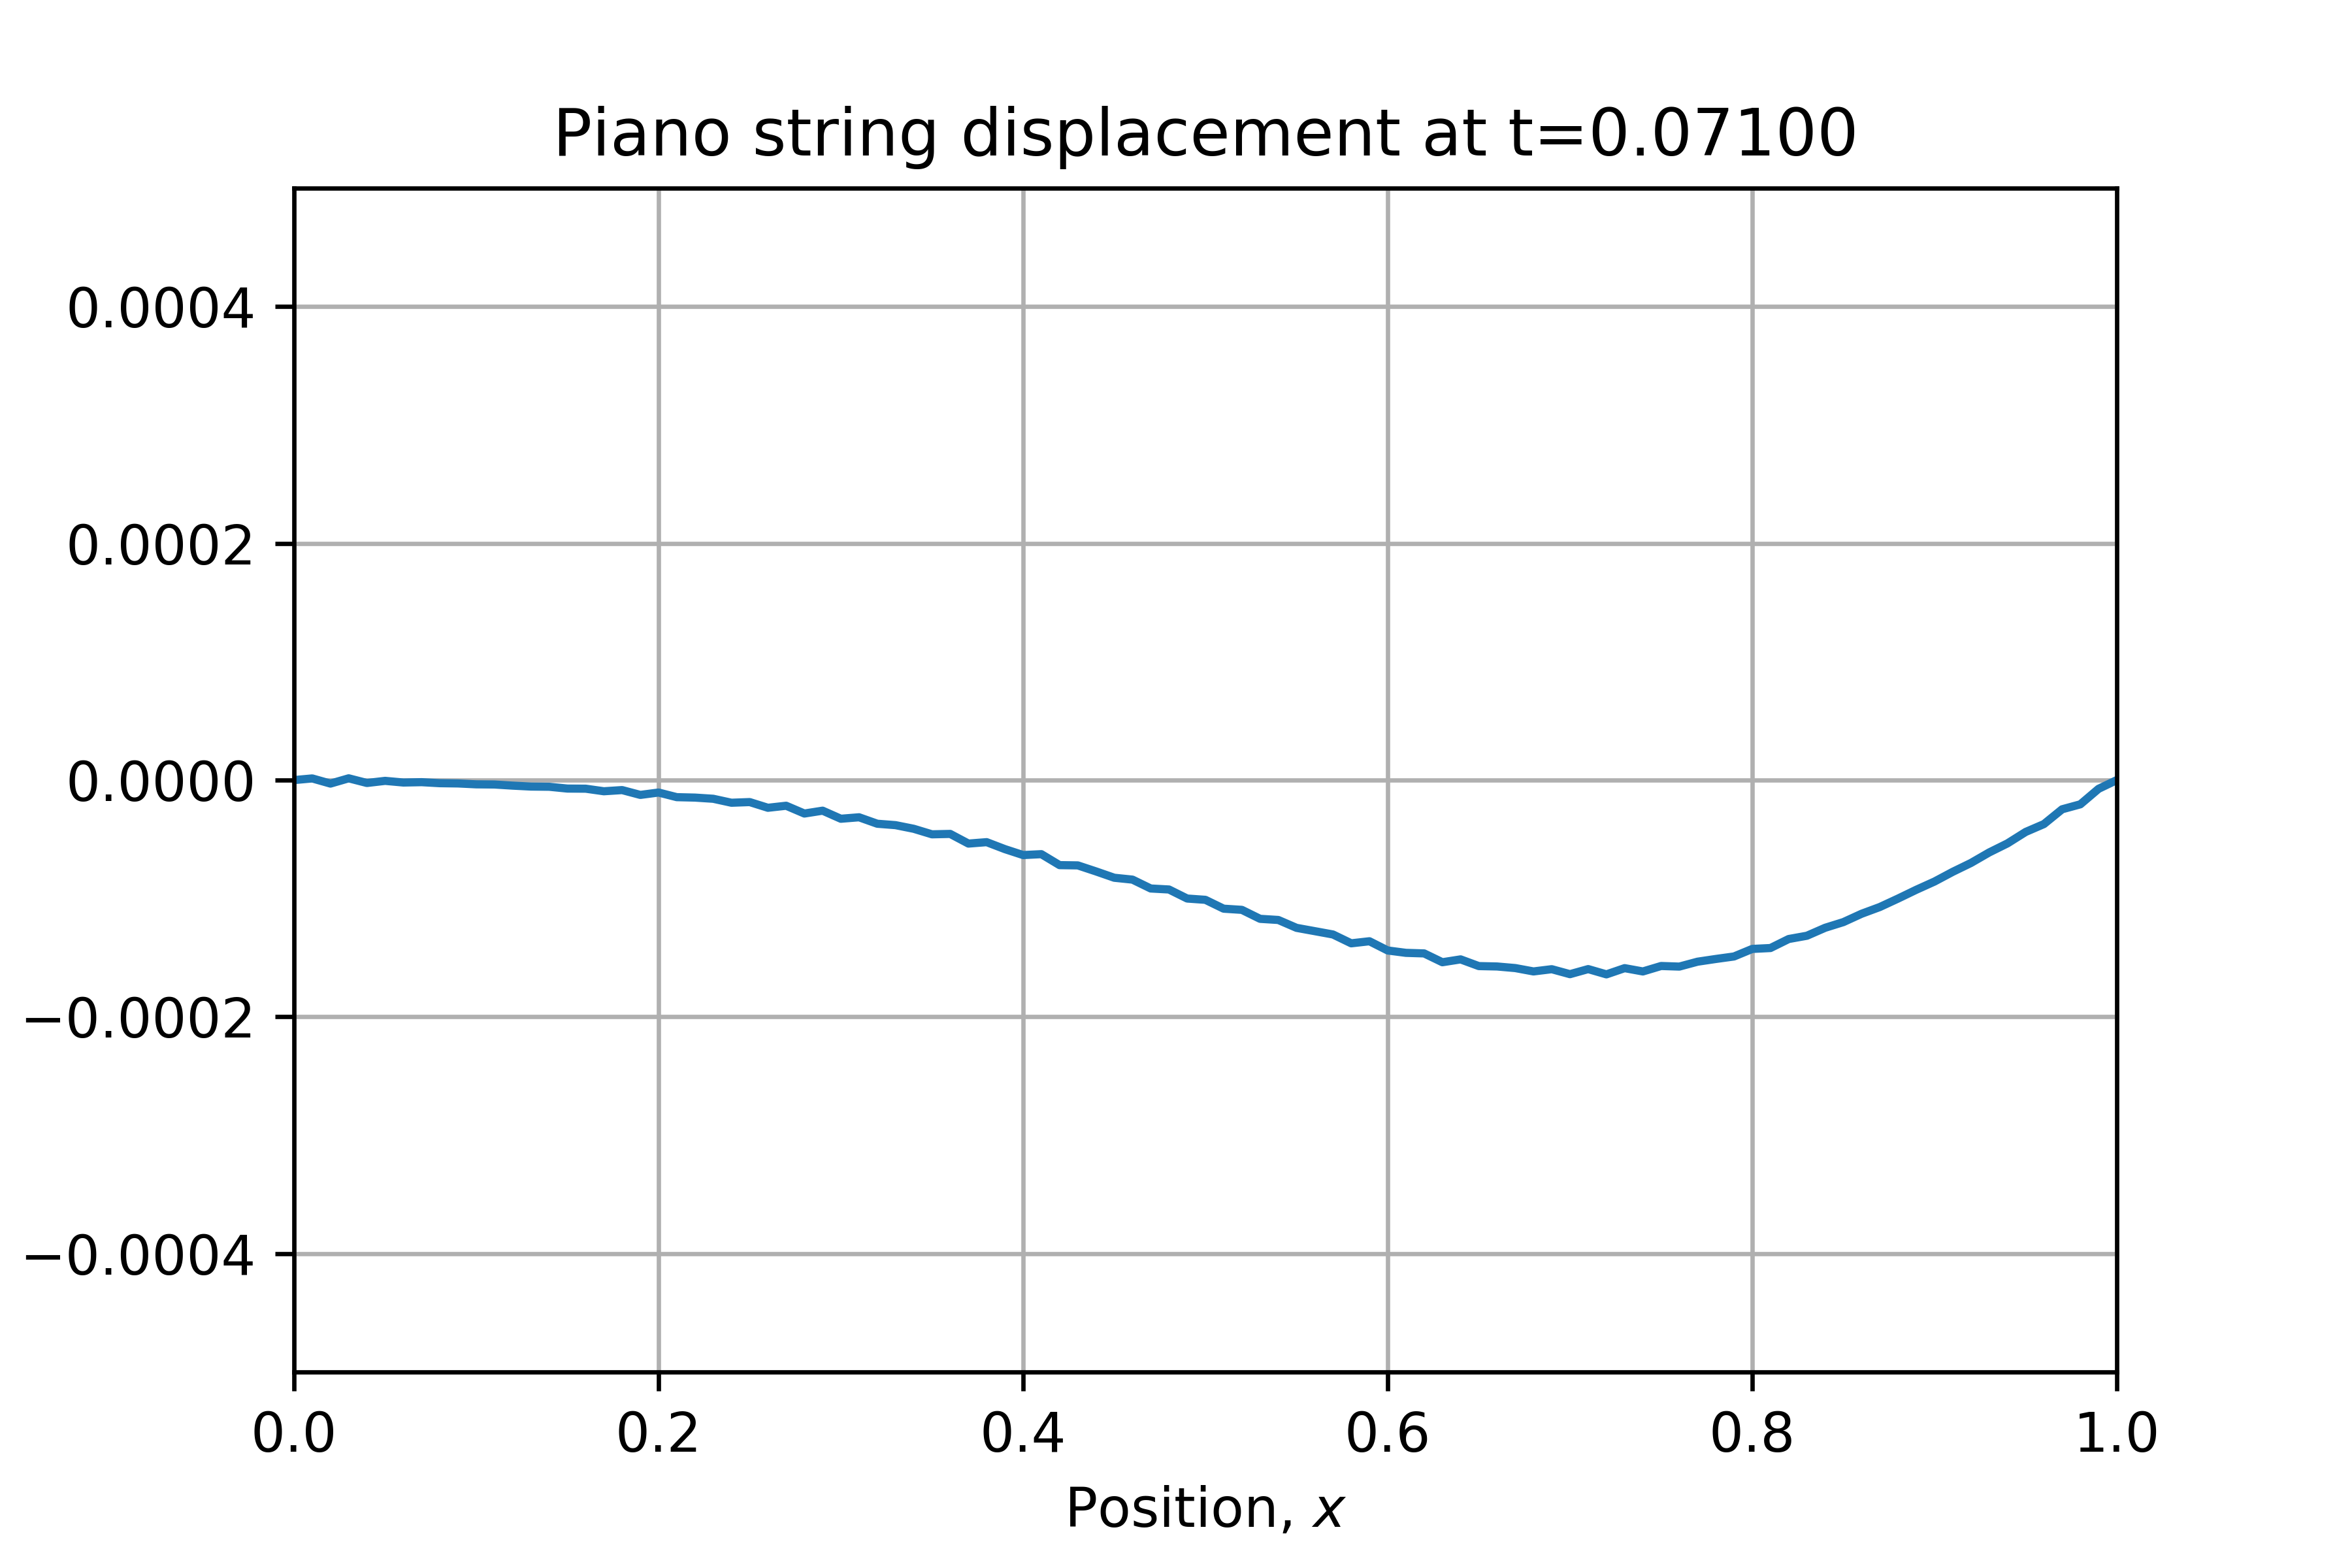
\includegraphics[width=0.8\textwidth]{../images/q2_plot_71.png}
	\caption{Plot of the piano string displacement at a time of 71ms.}
	\label{fig:q2_71}
\end{figure}

\begin{figure}[H]
	\centering
	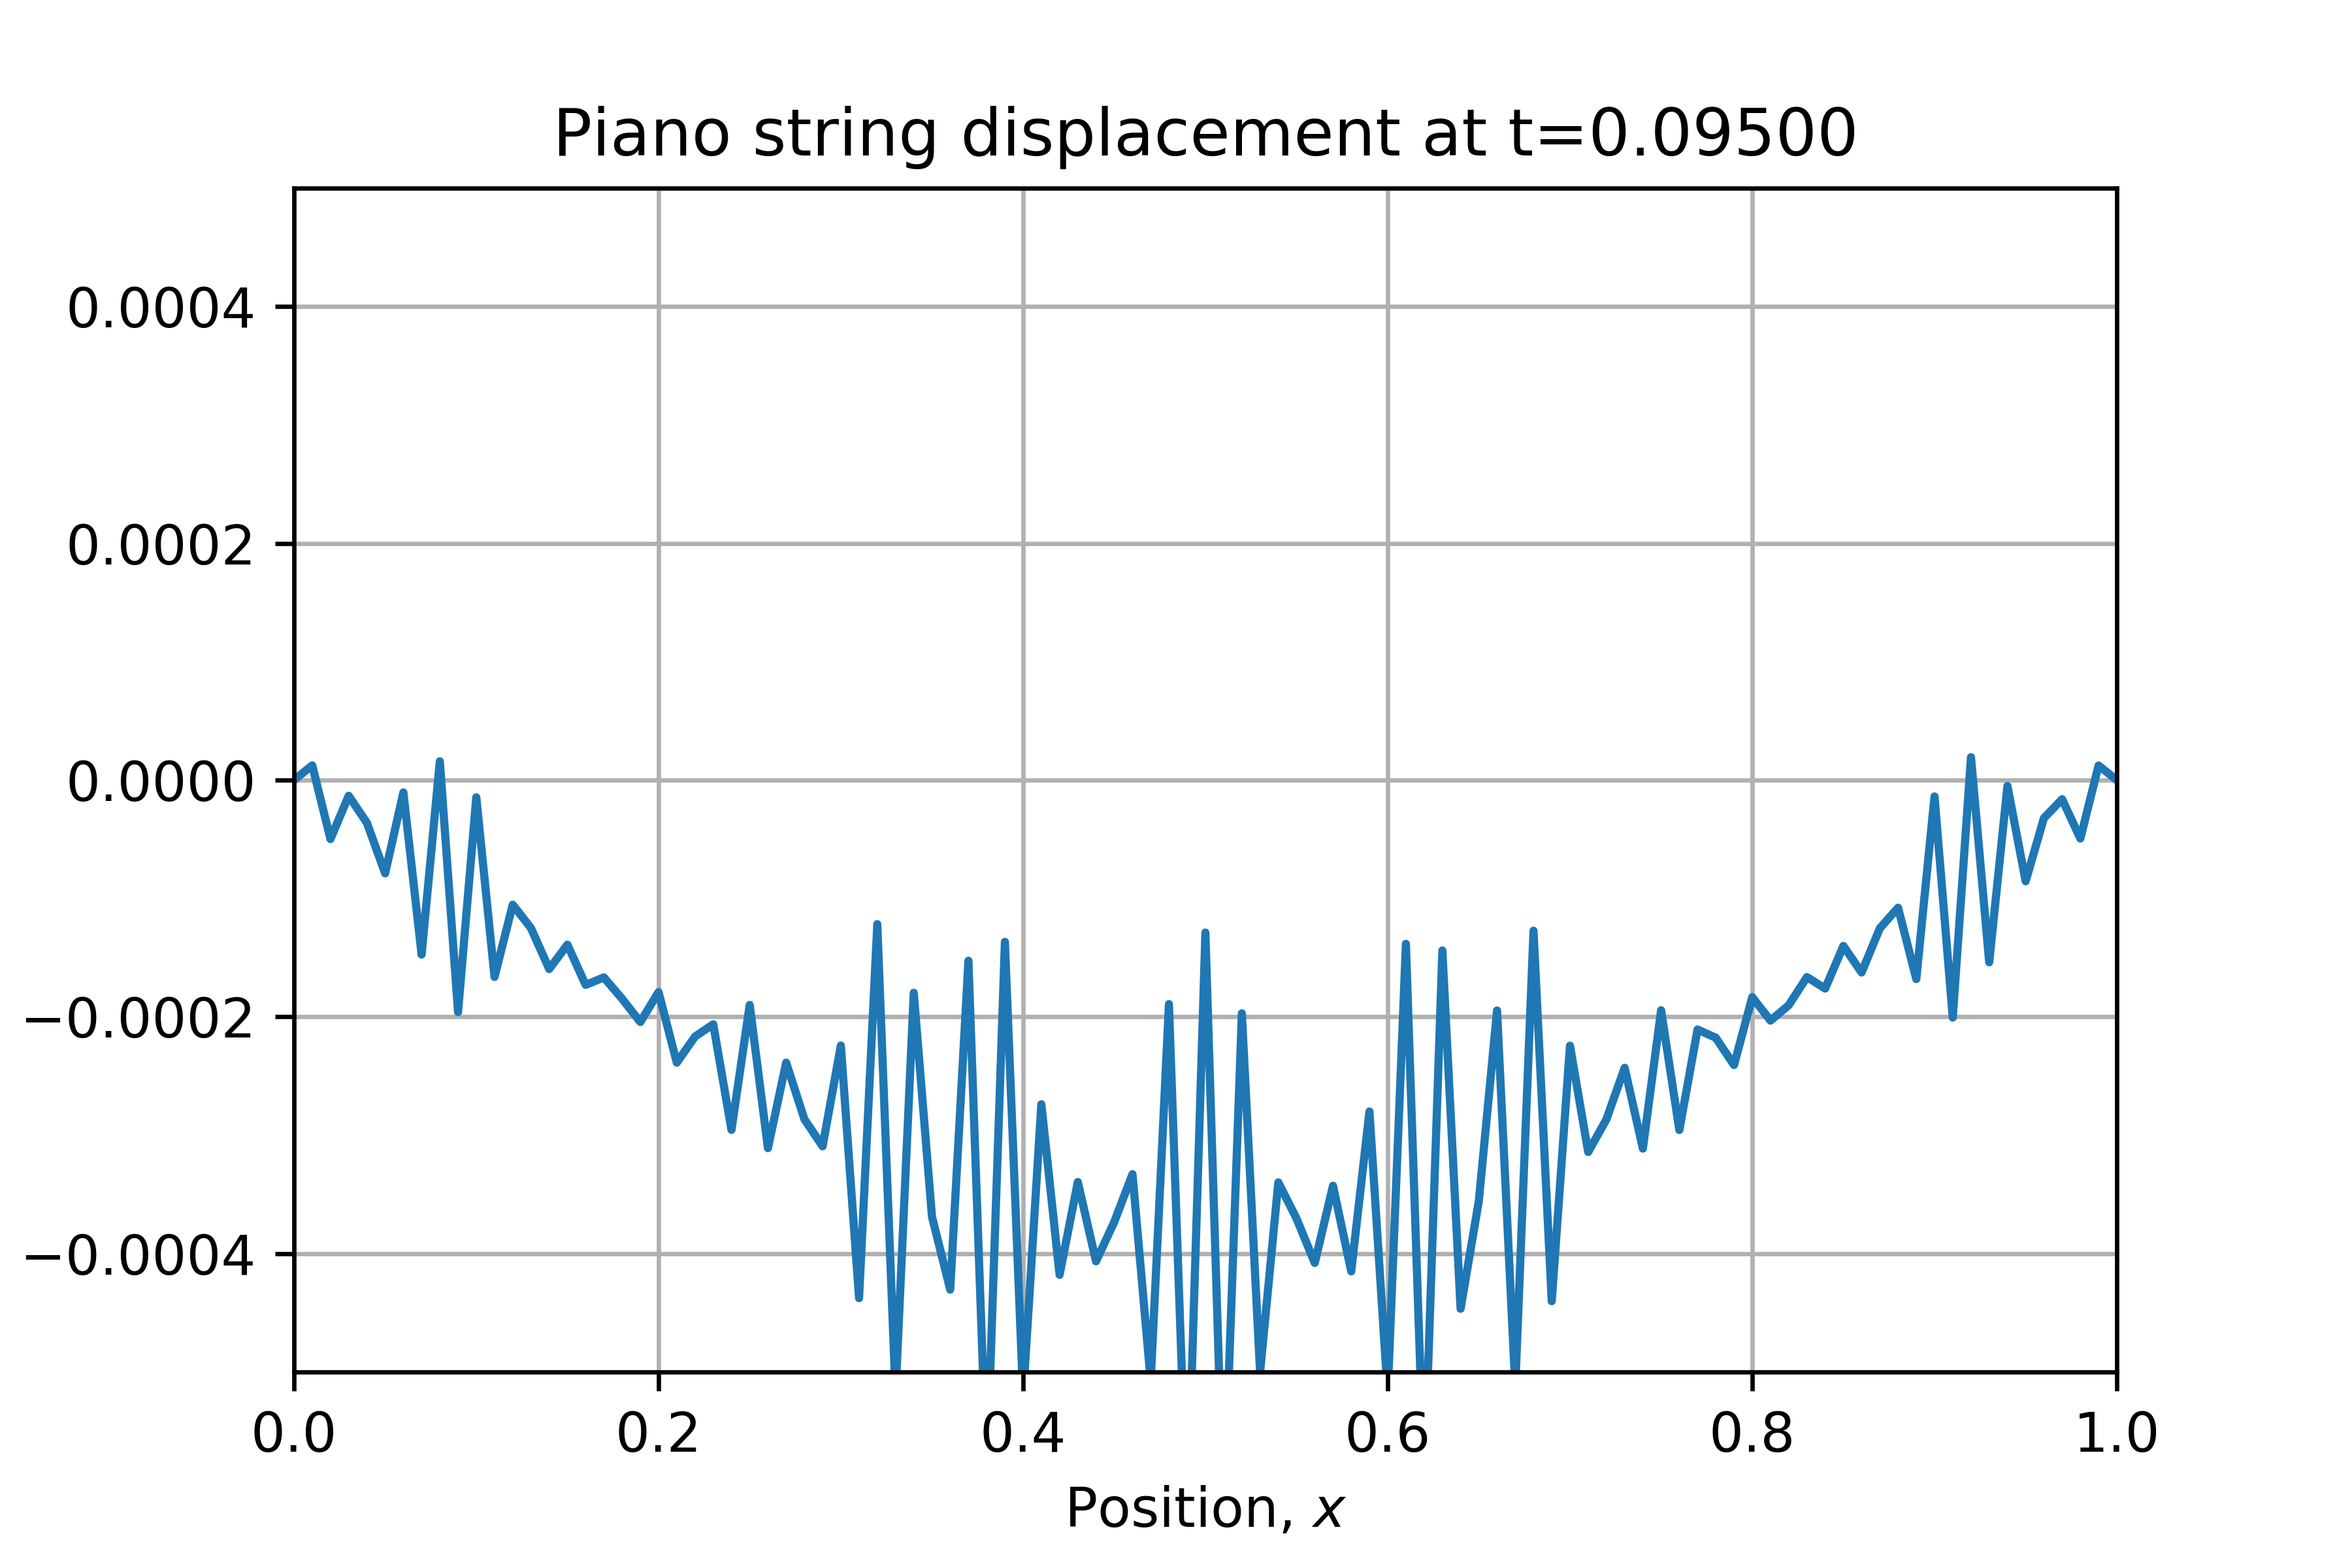
\includegraphics[width=0.8\textwidth]{../images/q2_plot_95.png}
	\caption{Plot of the piano string displacement at a time of 95ms.}
	\label{fig:q2_95}
\end{figure}

\begin{figure}[H]
	\centering
	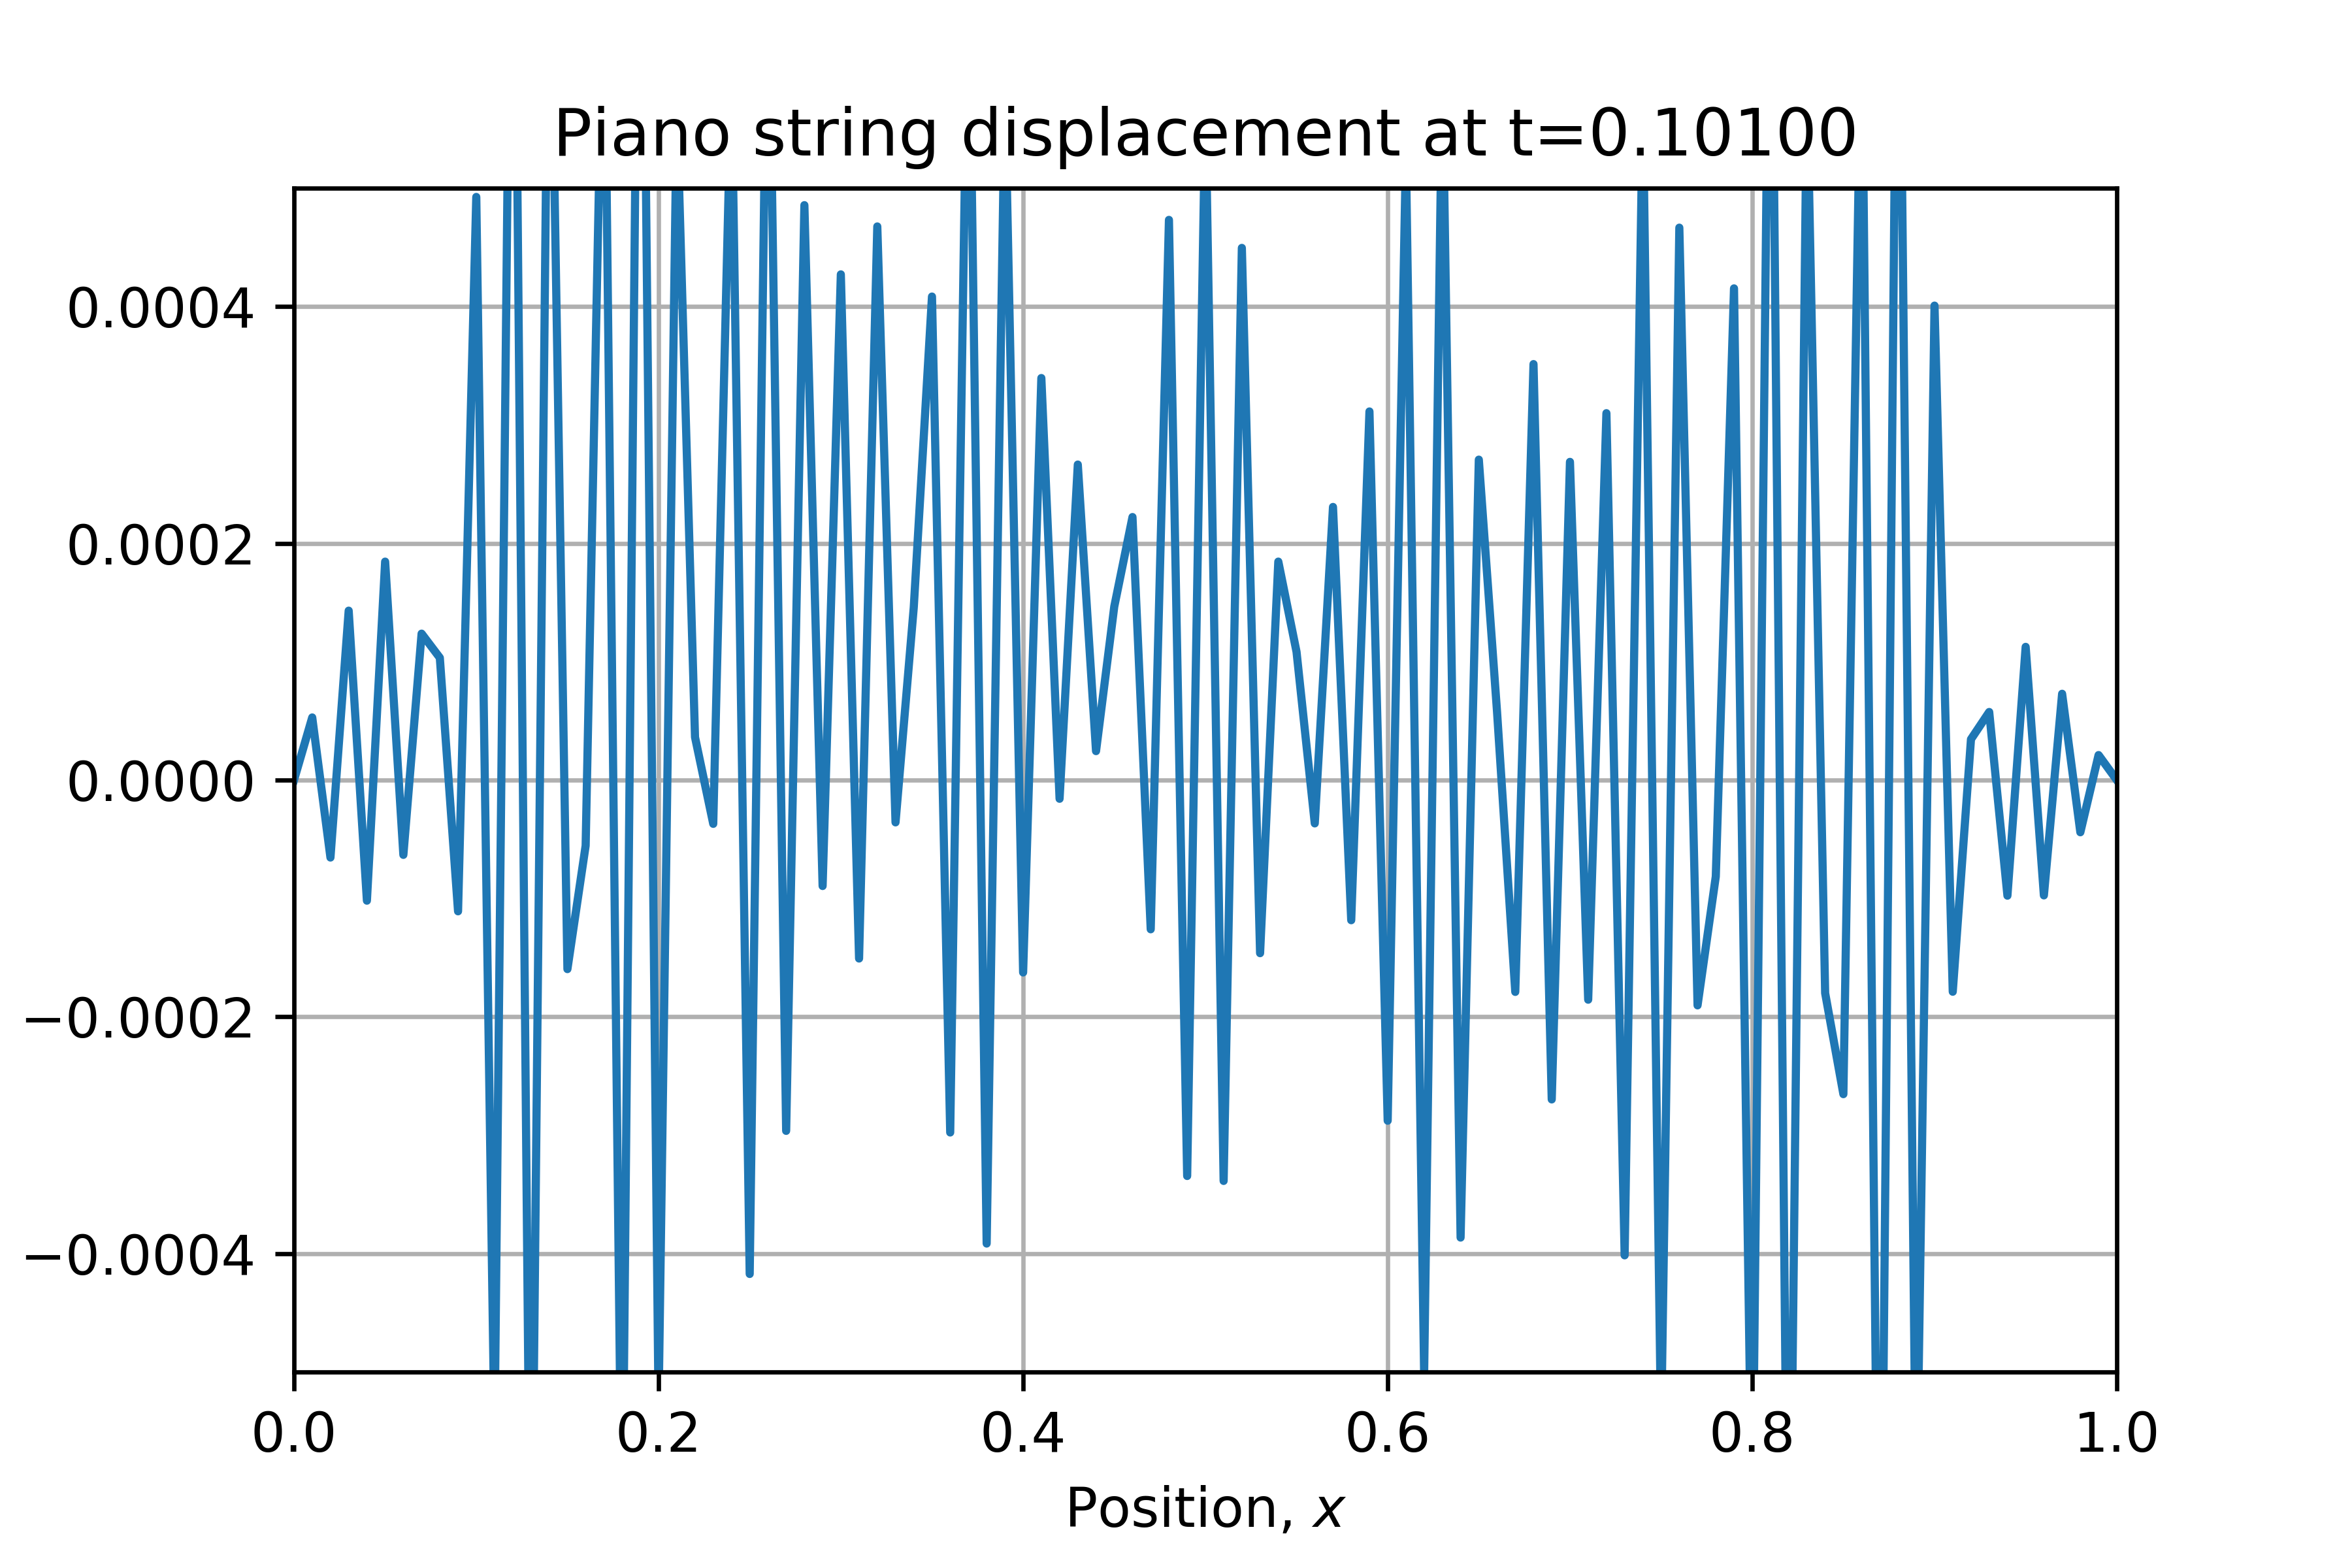
\includegraphics[width=0.8\textwidth]{../images/q2_plot_101.png}
	\caption{Plot of the piano string displacement at a time of 101ms.}
	\label{fig:q2_101}
\end{figure}


\section{Solving Burger's equation}
For this part of the lab we desire to solve Burger's equation

\begin{equation}
	\frac{\partial u}{\partial t} + \epsilon \frac{\partial}{\partial x}(\frac{u^2}{2}) = 0
\end{equation}

using Euler's method for an initial step forward and then using the leapfrog method.
Using the notation $u^j_i = u(x_i, t_j)$ where $x_i = i\Delta x$ for $i=0,...,N_x-1$, $\Delta x=0.02$ and $t_j = j\Delta t$ for $j=0,...,N_t-1$, $\Delta t=0.005$, the Euler step is performed using the equation

\begin{equation}
	u^1_i = u^0_i - \Delta t\epsilon u^0_i\frac{\partial u^0_i}{\partial x}
\end{equation}

and the subsequent leapfrog method is applied using

\begin{equation}
	u^{j+1}_i = u^{j-1}_i - \frac{\epsilon\Delta t}{2\Delta x}((u^j_{i+1})^2 - (u^j_{i-1})^2)
\end{equation}

The values used in our solution were $\epsilon = 1.0$, $L_x = 2 \pi $, $T_f = 2$, $N_x = integer(\frac{L_x}{\Delta x})$, $N_t = integer(\frac{T_f}{\Delta t})$ with initial condition $u(x, t=0)=\sin(x)$ and boundary condition $u(x=0,t)=0=u(x=L_x,t)$.
The solution of Burger's equation is plotted for times: $t=0.0,0.5,1.0,1.5$ shown in figure \ref{fig:burgers_even}.
From our solution we can see that as time progresses there's a shock formation around the mid point $x=Lx/2$, resulting in our initial sine function to become a sawtooth wave function. As time progresses we can see the formation of noise fluctuations approaching the shock ($x=Lx/2$) from both sides which we deemed to be unrealistic features of the solution. These noise fluctuations seem to be due to the method implemented to solve Burger's equation. This point becomes evident when we once again plotted the solution but increased the value of $N_x$ by one, shown in figure \ref{fig:burgers_odd}. This small increase resulted in a magnification of the noise. Furthermore, whenever $N_x$ was altered to be even the resulting solution matched that of figure \ref{fig:burgers_even} and whenever it was alter to be odd the resulting solution matched that of figure \ref{fig:burgers_odd}. Thus the noise was deemed to be due to the leapfrog method and fixed time steps used to solve the equation. Lastly we decreased the step sizes $\Delta x$ and $\Delta t$ by an order of magnitude and observed a dampening of this noise of the method implemented. The damped version of our original solution is shown in figure \ref{fig:burgers_damped}. 

\begin{figure}[H]
	\centering
	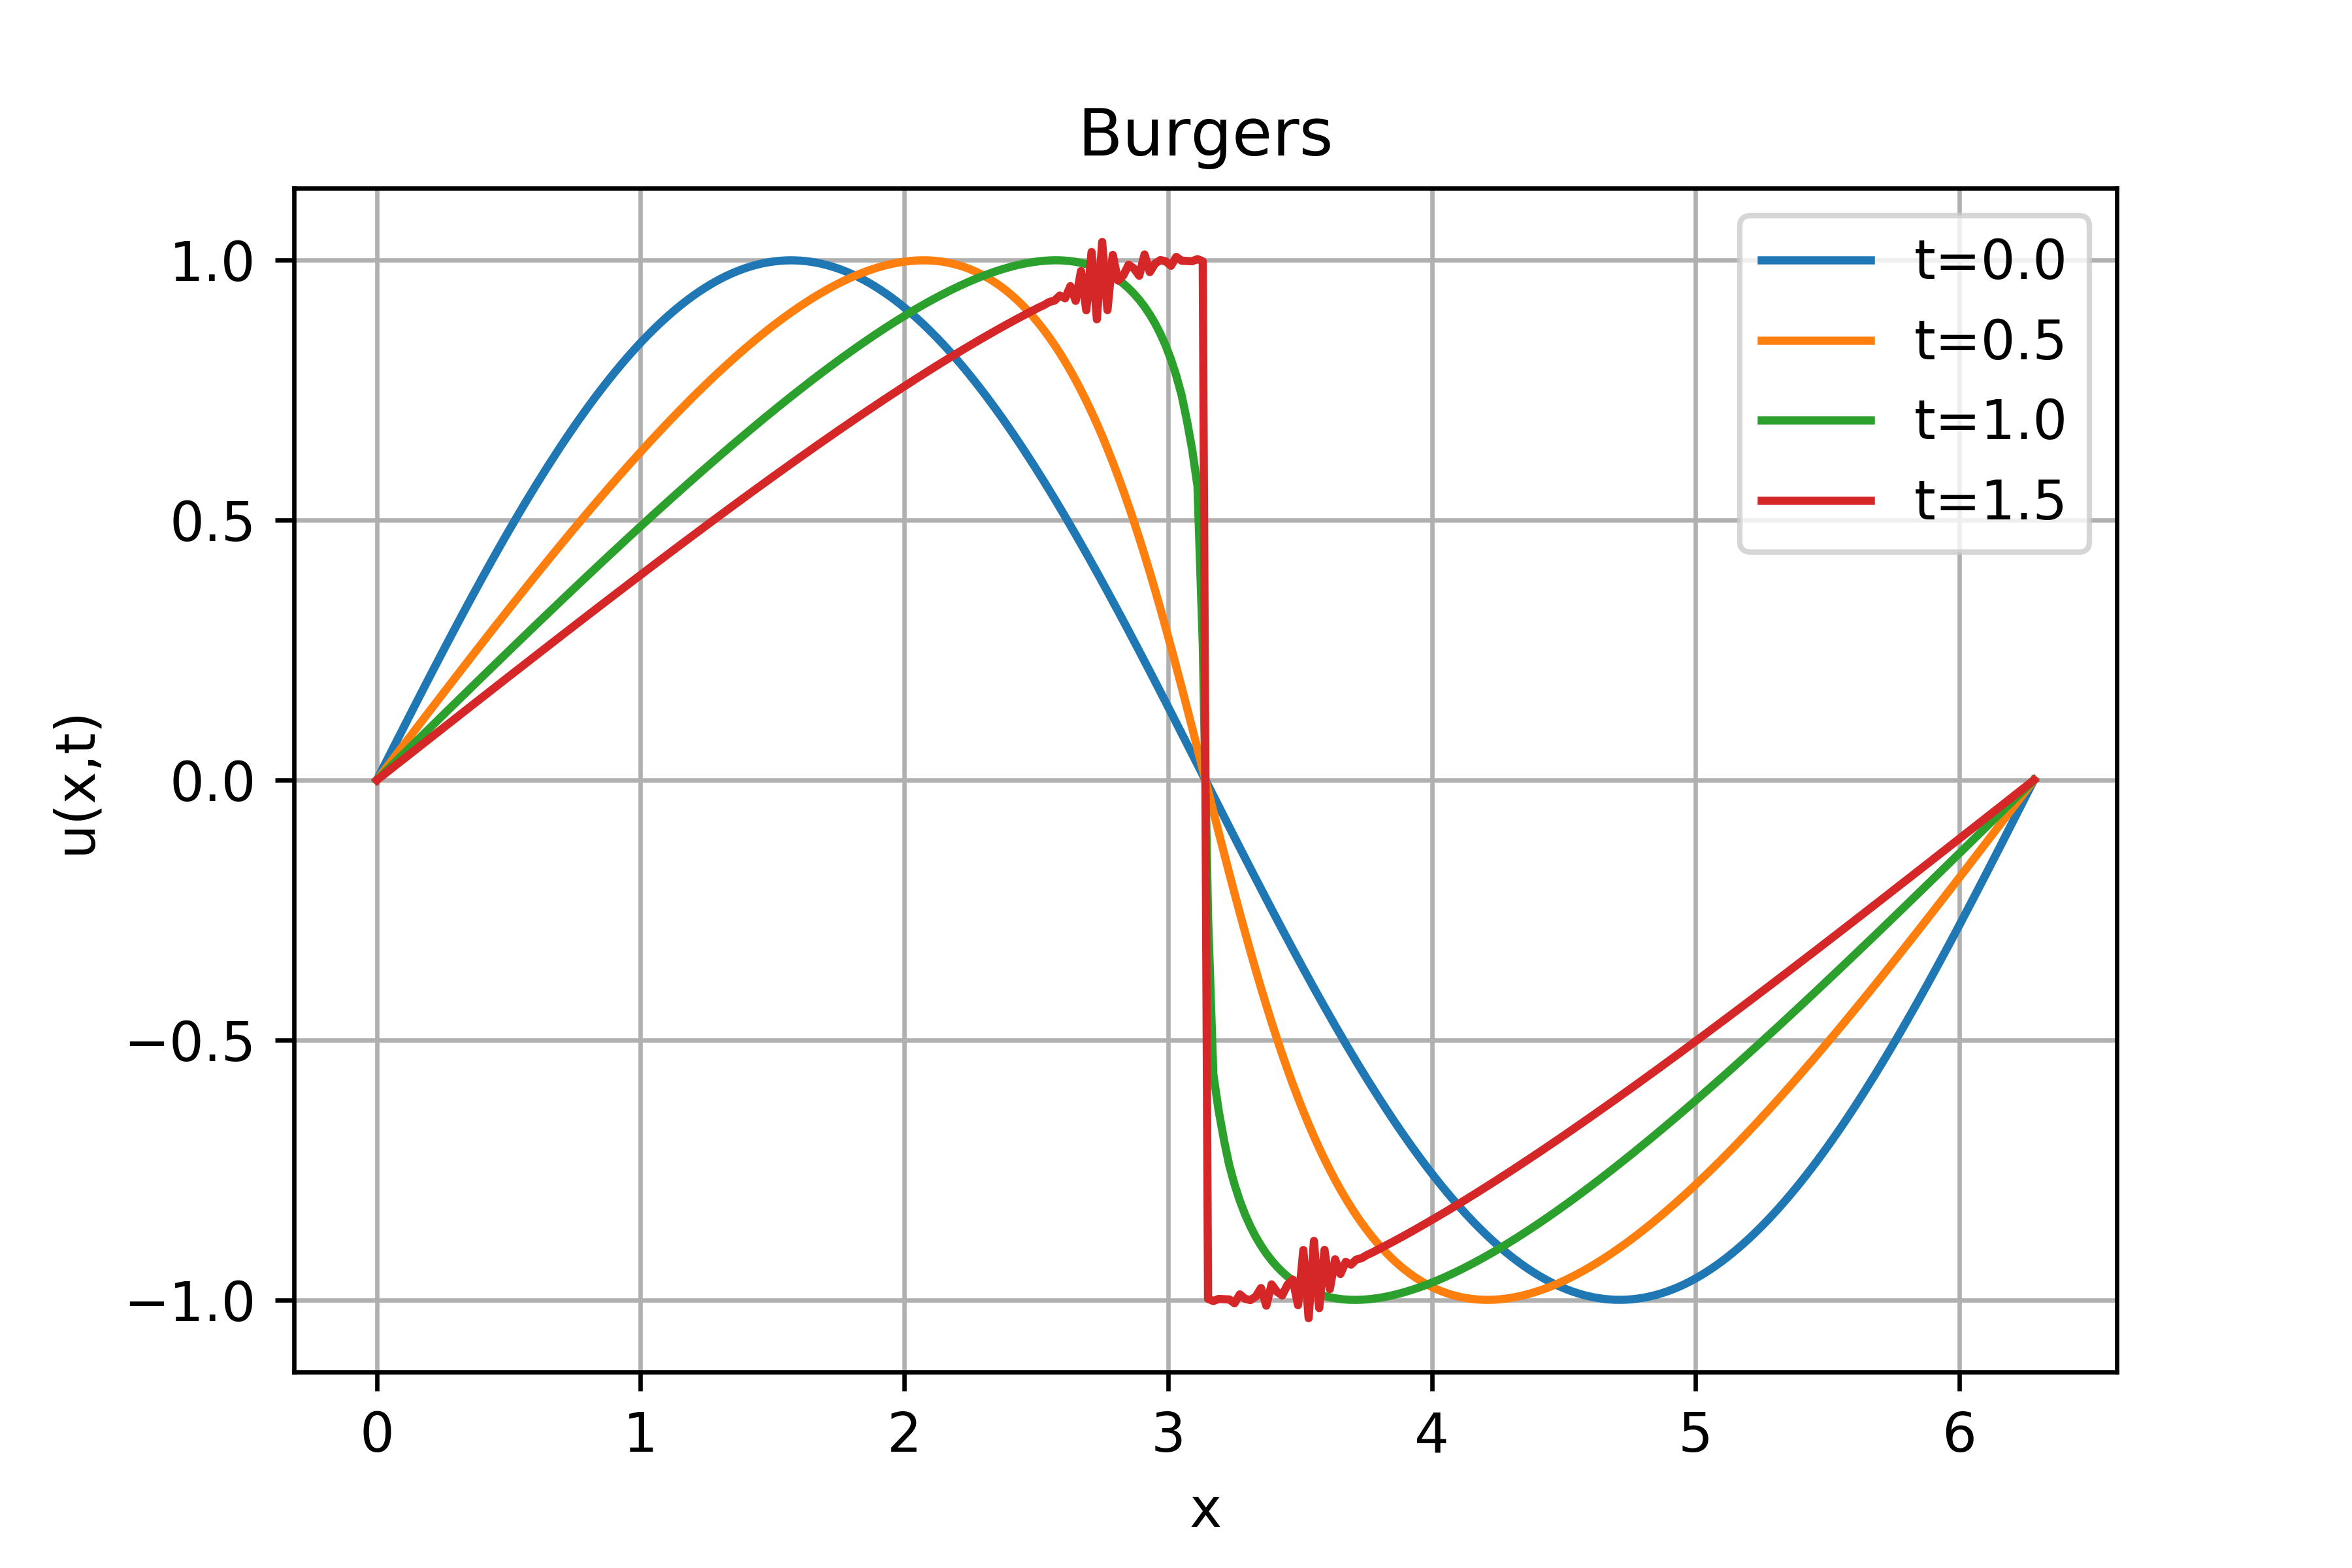
\includegraphics[width=0.8\textwidth]{../images/burgers.png}
	\caption{Plot of the solution of Burger's equation for times $t=0.0,0.5,1.0,1.5$ using an even number of points, $N_x=314$, with $\Delta x=0.02$ and $\Delta t=0.005$}
	\label{fig:burgers_even}
\end{figure}

\begin{figure}[H]
	\centering
	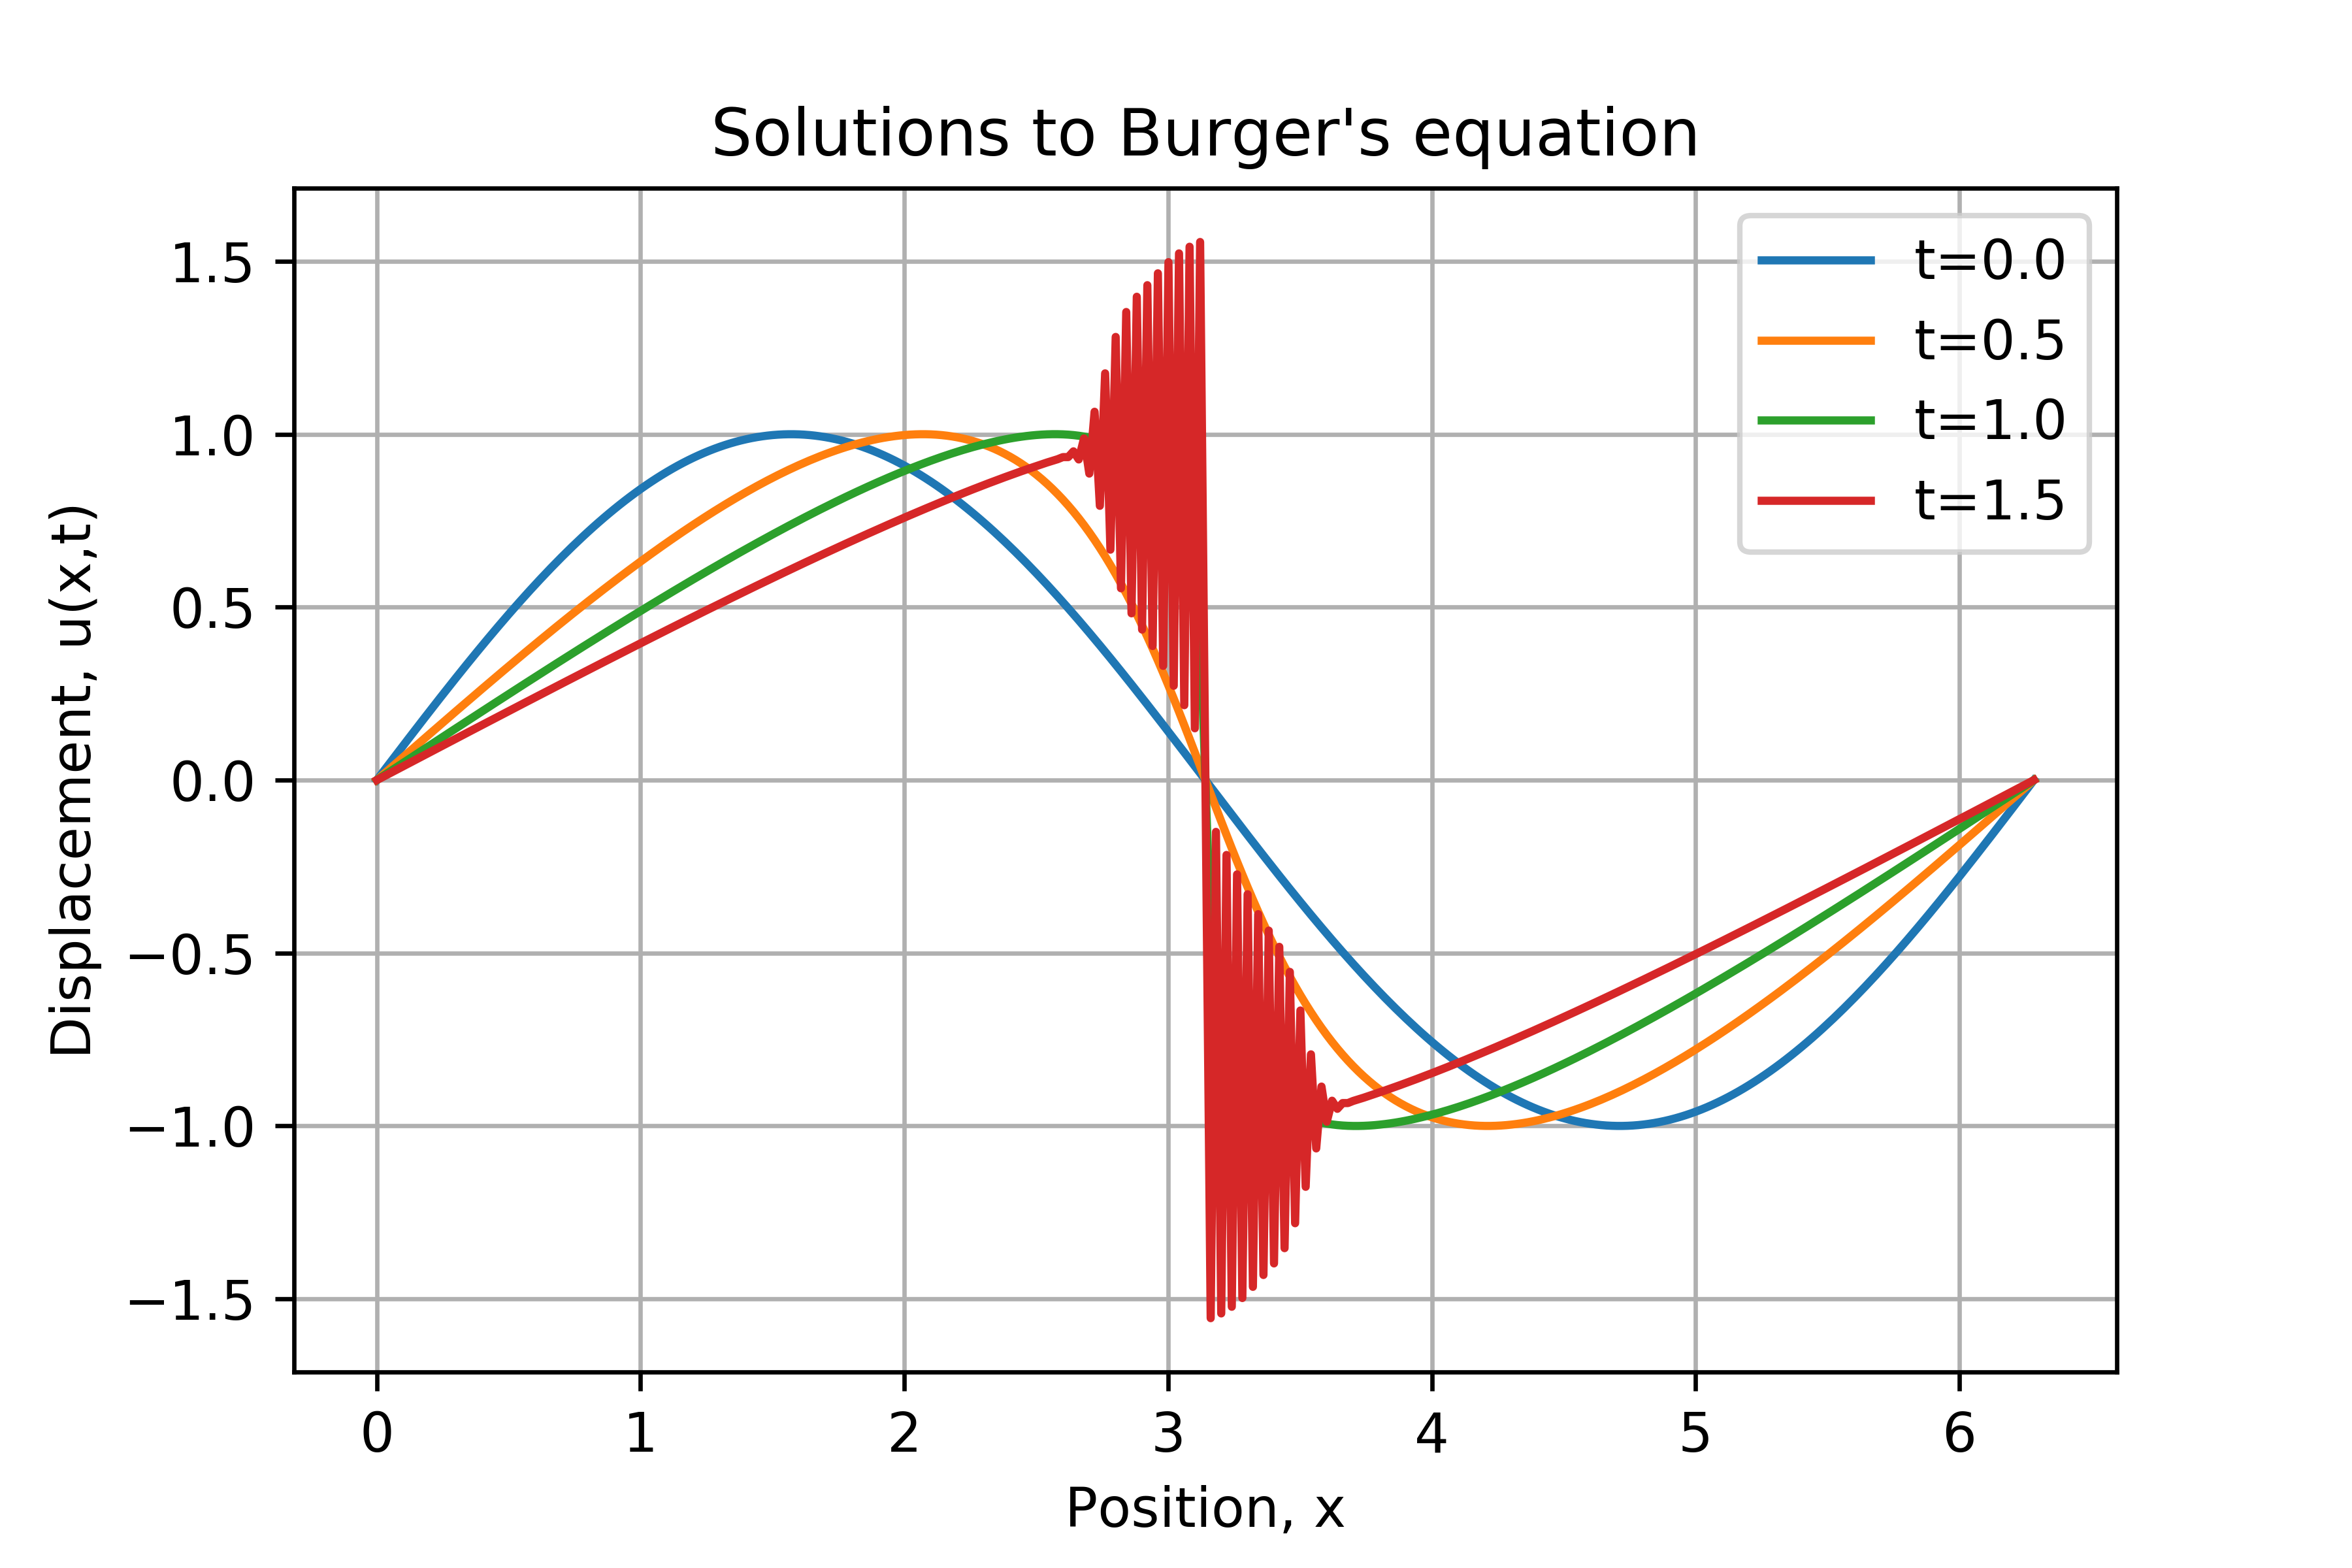
\includegraphics[width=0.8\textwidth]{../images/burgers_odd.png}
	\caption{Plot of the solution of Burger's equation for times $t=0.0,0.5,1.0,1.5$ using an odd number of points, $N_x=315$, with $\Delta x=0.02$ and $\Delta t=0.005$}
	\label{fig:burgers_odd}
\end{figure}

\begin{figure}[H]
	\centering
	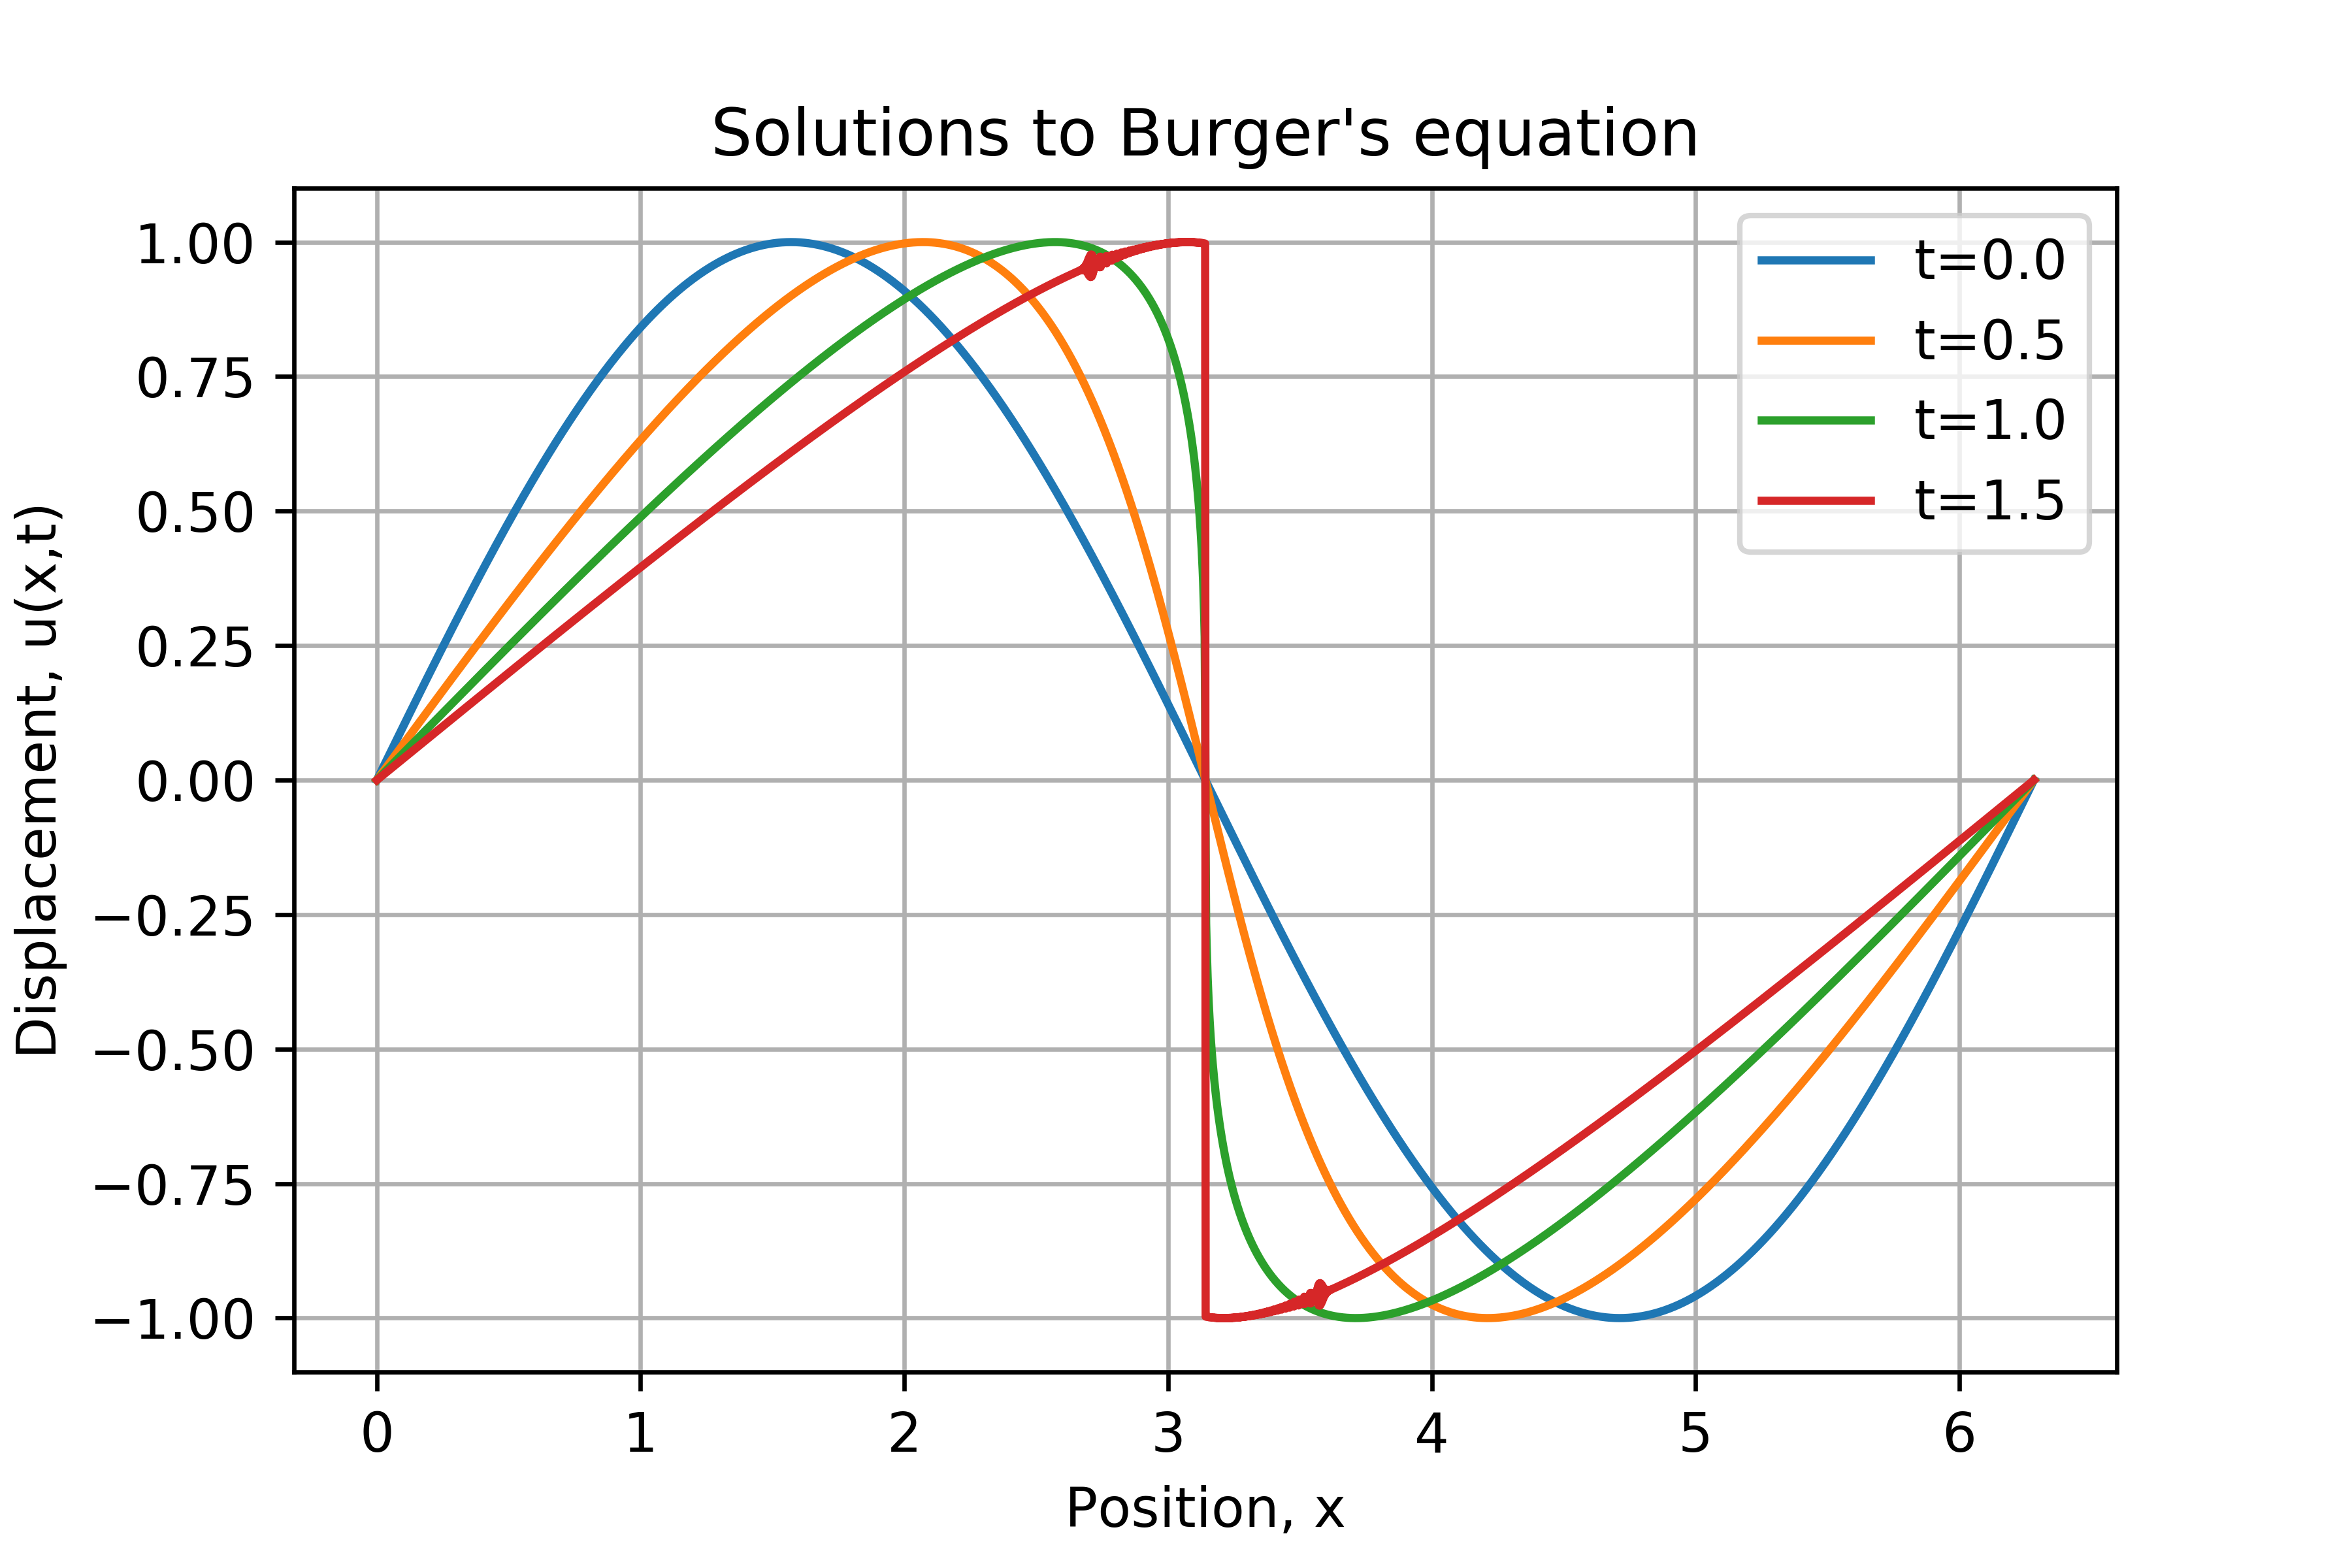
\includegraphics[width=0.8\textwidth]{../images/burgers_damped.png}
	\caption{Plot of the solution of Burger's equation for times $t=0.0,0.5,1.0,1.5$ using step sizes that are an order of magnitude smaller $\Delta x=0.0019$ and $\Delta t=0.000476$, with even number of points, $N_x=3298$. The noise in the solution can be seen to dampen out when compared to that of figure \ref{fig:burgers_even}}
	\label{fig:burgers_damped}
\end{figure}
\end{document}